%% This LaTeX-file was created by Marco Kienzle (Marco.Kienzle@gmail.com)
%% 
%% Do not edit this file unless you know what you are doing.

% This latex template was created to produce document that will be transformed into MS Word document.
% The command to do so is 
% latex article.tex
% bibtex article
% latex2rtf -Z3 -P /usr/local/share/latex2rtf/cfg/:/tmp/latex2rtf-1.9.16a/scripts/ article.tex

\documentclass{article}
%\documentclass{nrc2}
%\journal{cjfas}

\usepackage[dvips]{color}

\usepackage{bbding}
\usepackage{natbib}
\usepackage{setspace}
\usepackage{amsmath}
\usepackage{graphicx}
%\usepackage{psfig}
\usepackage{verbatim}
\usepackage{rotating}
\usepackage{multirow}
\usepackage{longtable}
\usepackage{booktabs}
\usepackage{subfigure}
\usepackage{lineno}

\setlength{\oddsidemargin}{0.5cm}
\setlength{\evensidemargin}{0.5cm}
\setlength{\textwidth}{17cm}
%\setlength{\textheight}{23cm}
%\addtolength{\oddsidemargin}{-3cm}
%\addtolength{\evensidemargin}{-3cm}

\begin{document}

\linenumbers

\title{Yet another general theory for the analysis of catch at age data: \\ applying survival analysis to fisheries research}

\author{Marco Kienzle\footnote{DAFF biometry, Brisbane, Queensland, Australia} and Nicole White\footnote{QUT, Brisbane, Queensland, Australia}}

\maketitle

%\tableofcontents

%\abstract{Fisheries management agencies around the world collect age data for the purpose of assessing the status of natural resources in their juridiction. Estimates of mortality rates are central to assess the sustainability of fish stocks exploitation. Survival analysis has seldom been applied to fisheries research despite its widespread use in medical research and engineering to estimate failure rates. In this paper, we present a variety of hazard functions to model the dynamic of a fishery and estimate by maximum likelihood all parameters necessary for a stock assessment (including natural and fishing mortality rates as well as gear selectivity) from a sample of fish age. These methods were tested by Monte Carlo simulations to assert that they provide un-biased estimates of these quantities. An application to the Queensland's sea mullet fishery (Australia) dataset provided an estimate of natural mortality equal to 0.319 $\pm$ 0.165 year$^{-1}$.


%% Survival analysis has seldomed be used in this area of research despite estimate fish mortality ratesSurvival analysis was applied to fisheries catch at age data to develop maximum likelihood estimators for stock assessment. This new method estimated natural mortality, fishing mortality and catchability from typical catch at age matrices. Monte Carlo simulations suggested estimates were unbiased and provided a better fit than the traditional multinomial approach. 

%% Application to a dataset from Queensland's sea mullet fishery (Australia) estimated natural mortality to be equal to 0.319 $\pm$ 0.165 year$^{-1}$.
}

%\clearpage
%\newpage
%\pagecolor{blue}

%\textcolor{white}{test}

\section{Introduction} One of the purposes of stock assessment is to estimate mortalities affecting fish stocks. This task is much easier for species that can be aged compared to, for example crustaceans, which aging is not possible. The reason lies in that mortality and longevity are inversely related hence age is a measure, albeit inverse, of mortality. The central mortality model used in fisheries research was proposed by Baranov to describe the variation of the number of fish belonging to a cohort through time \citep{quin99b}. This deterministic exponential model has a statistical counterpart in the form of the exponential probability distribution function which first and second moments quantify the relationship between longevity (age) and mortality rate \citep{cow98b}. Adopting a statistical view of this problem allowed to develop maximum likelihood estimators \citep{Burnb03} of parameters of importance to stock assessment scientists. The branch of statistics focused on survival analysis has created and refined methods to estimate mortality rates \citep{cox84b} which are widely applied in the fields of medical research and engineering. \\ 

%The present article describes an application of survival analysis to fisheries catch at age data.
Despite the commonalities between survival analysis for medical and fisheries research, this theory has seldom been applied to animal ecology \citep{Pollock1989}: to our knowledge, there hasn't been any application to fish age data for the purpose of stock assessment. In this manuscript, we described how to apply survival analysis to create likelihood functions of catch at age for the purpose of estimating natural and fishing mortalities as well as gear selectivity. We started with a simplistic example of constant natural and fishing mortality to introduce fundamental concepts from survival analysis before moving to more sophisticated cases leading to its application to real data from the sea mullet fishery in Queensland (Australia). The proposed methods were tested with simulated data to characterize some of their properties and their capacity to estimate population dynamic parameters of interest. Finally, the application to the mullet fishery case study provided specific estimates of natural mortality, catchability and selectivity. \\


\section{Survival analysis} 
%\subsection{Properties of the exponential pdf}
% which properties inversily relate mortality rates to the average (and dispersion) of age in a cohort (CITE Keith Brander)

\subsection{Abundance of individual belonging to a cohort} \input{/home/mkienzle/mystuff/Work/Theory_for_fisheries/Writing/FishingASingleCohort.tex}

\subsection{Survival analysis approach to single cohort}

The exponential decrease in abundance of a fish cohort is described in survival analysis \citep{cox84b} using a constant harzard function of time ($t$) and parameters $\theta$

\begin{equation}
h(t; \theta) = M + F
\end{equation}

It follows that the density function is:

\begin{equation}
f(t; \theta) = (M + F) \ e^{-(M+F)t}
\end{equation}

The survivor function gives the proportion of cohort surviving longer than $t$ \citep{kleinbaum2005survival}
\begin{equation}
P(T>t) = S(t; \theta) = e^{-(M+F)t}
\end{equation}

Finally, the cumulative distribution function $F(t)$ with density $f(t)$ gives the proportion of the cohort that died until time $T=t$
\begin{equation}
F(t) = 1 - S(t)
\end{equation}

The probability of dying between $t_{1}$ and $t_{2}$ is
\begin{equation}
P(E_{[t_{1}-t_{2}]}) = \int_{t_{1}}^{t_{2}} f(t; \theta) = F(t_{2}) - F(t_{1}) = S(t_{1}) - S(t_{2})
\end{equation}

The total number of individuals that die in an interval ($E_{[t_{1}-t_{2}]}$) is made of those that were caught in the interval ($C_{[t_{1}-t_{2}]}$) plus the number of individual dying of natural causes ($D_{[t_{1}-t_{2}]}$):  $E_{[t_{1}-t_{2}]} = C_{[t_{1}-t_{2}]} + D_{[t_{1}-t_{2}]}$

So, survival analysis provides the tools to build a likelihood estimator of mortality rates. Let's take the same example as above, supposing that we have access to the number of individual dying in each interval. In the R script below, we implicitly assume a knowledge of likelihood for binned data \citep{cow98b}

\verbatiminput{SimplestExample.R}

This simplistic example above illustrates the usage of survival analysis. It suffers from several shortcomings that we will address one by one to apply survival analysis to fisheries catch at age data. In principle, survival analysis offers the tools to represent any mortality schedule and the likelihood approach provides a method to compare them and determine which is most supported by the data.\\

First, we introduce the concept of truncated distributions to address the case where some age-groups are not samples, for example in Torres Strait lobster where age-group 2+ migrates outside the fishing grounds to Papua New Guinea to spawn.

\verbatiminput{TruncatedDistribution.R}

Second, total death data are not available to fisheries scientist. Instead, they are often provided with catch from a fishery. 

\verbatiminput{SimplestExampleUsingCatch.R}

Third, we would also to estimate natural mortality from catch at age data. This is possible if you have a measure of effort ($E$) and that it relates to fishing mortality via catchability ($q$): $F=qE$

\verbatiminput{../Scripts/HowToEstimateMandQfromCatchData.R}

Fourth, often gear properties interfere with the selection of fish caught.
\verbatiminput{../Scripts/HowToEstimateMQandSelectivity.R}

Finally, we can process data from several cohorts at the same time using the standard format of a catch at age matrix (year x age-groups). Multiplicity of data to estimate natural mortality, catchability and selectivity ( using the assumption of separability ) improves our capability substantially.
\verbatiminput{../Scripts/HowToEstimateqMAndSelectivityFromCatchAtAge.R}




%Similarities between the Baranov equation (Eq.~\ref{BaranovCatchEquation}) and the density function suggested that likelihood mortality rates could be estimated by maximum likelihood using catch data.

%% \subsection{Maximum likelihood with binned data}

%% In fisheries, age measurements are binned into age-groups spanning 1 year according to the annual deposit of material on otoliths. These annual rings allow to identify how many period of deposition each individual survived through. According to this observations, individual fish in a sample are classified into a discrete age-group ranging from 0 to a maximum age. Assuming age is distributed according to the density function $f(t; \theta)$, the probability to belong to an age-group $i$ is

%% \begin{equation}
%% \nu_{i} = \int_{i}^{i+1} f(t; \theta) dt
%% \end{equation}

%% And the log-likelihood function by \citep{cow98b}
%% \begin{equation}
%% {\rm log} L(\theta) = \sum_{i=0}^{N} n_{i} \ {\rm log} \ \nu(\theta)
%% \end{equation}

%\subsection{Numerical example}

%The following R script \citep{R} illustrates how likelihood estimates of mortality rates are obtained from this simple cohort catch data.
%\verbatiminput{../Scripts/HowToEstimateFfromCatchData.R}

%The following R script \citep{R} illustrates how catchability and natural mortality (M) are estimated providing effort is given
%\verbatiminput{../Scripts/HowToEstimateMandQfromCatchData.R}

%The following R script \citep{R} illustrates how catchability and natural mortality (M) are estimated from a catch at age matrix providing effort is given
%\verbatiminput{../Scripts/HowToEstimateqAndMFromCatchAtAge.R}


%\section{Materials and methods} 

%   \subsection{Data} \input{data.tex}

%   \subsection{Moreton Bay trawl fishery} \input{MoretonBaySandCrabFishery.tex}

%\section{Results}

%   \subsection{Fishery statistics} \input{ResFisheryStats.tex}

%\section{Results} 
% ---> did you observed catch in winter being lower than in summer ? if so by how many percent ?
%\input{}

\clearpage
\newpage
%% %% Bibliography
\bibliography{a-JLong,Biblio}
%\bibliographystyle{plain}
\bibliographystyle{plainnat}
%\bibliographystyle{abbrv}
%\bibliographystyle{apalike}

\clearpage
\newpage
\section*{Figures}

%% Illustration of exponential decay with constant mortality
 \begin{figure}[!ht]
%     \includegraphics[scale=0.6, angle = -90]{/home/mkienzle/mystuff/Work/Theory_for_fisheries/Writing/Graphics/IllustrationOfExpDecay.ps}
     \includegraphics[scale=0.6, angle = -90]{Graphics/IllustrationOfExpDecay.ps}
      \caption{An illustration of the decreasing number of individual in a cohort, assuming $Z = 0.6$ years$^{-1}$ and N$_{0}=1000$.}
     \label{fig:IllustrationOfExpDecay}
   \end{figure}

%\clearpage
%\newpage
%\section*{Tables}

%\clearpage
%\newpage
%\section*{Programs code}

\end{document}









